\section{Context}
This thesis sprung from the participation of a team of students to the the "Robocup" contest. Robocup is a robotic contest in which robots from all around the world compete in a game of football. There are various categories but our team will compete in the kidsize competition.

\begin{figure}[htp]
\center
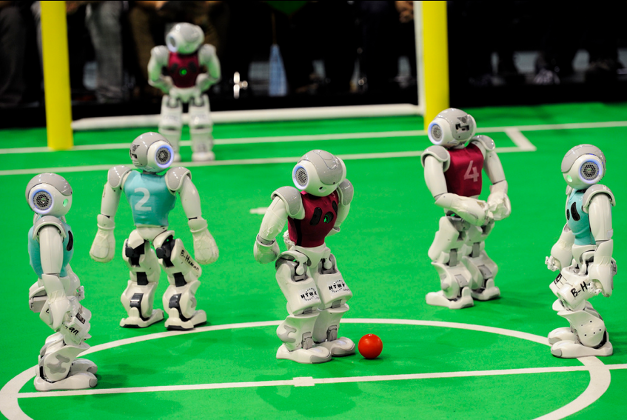
\includegraphics[width=0.5\textwidth]{figures/robocup}
\caption[Two teams of Nao robots playing against each other]{Two teams of Nao robots playing against each other in the 2014 edition of RoboCup \textit{[Photo courtesy of RoboCup]}}
\label{fig:intro_robocup}
\end{figure}

\section{Scope}
The scope of this thesis is to provide the team with a simulation tool and a model able of :
\begin{itemize}
\item simulating realistic inertias
\item receiving orders at approximately 300Hz
\item simulating friction realistically
\item incorporating springs and dampers
\item visualization
\end{itemize}

The model should also receive the same orders as the real robot.
